\documentclass{article}

\usepackage{graphicx}
\usepackage{amsmath}
\usepackage{caption}
\usepackage{subcaption}
\usepackage{listings}
\usepackage[hidelinks]{hyperref}
\usepackage{enumitem}
\usepackage{geometry}
\usepackage{biblatex}
\usepackage{wrapfig}
\usepackage[entrycounter=true]{glossaries}

\makeglossaries

\newglossaryentry{aggregate}
{
    name=aggregated,
    description={The process of combining individual votes to produce a summary count or total that reflects the collective outcome of the election.}
}

\newglossaryentry{audit}
{
    name=audit,
    description={The systematic review and verification of the voting process and results to ensure the accuracy, integrity, and transparency of an election.}
}

\newglossaryentry{authentication}
{
    name=authentication,
    description={The process of verifying the identity of a voter before they are allowed to cast a vote.}
}

\newglossaryentry{encapsulate}
{
    name=encapsulated,
    description={The process of representing all the relevant data about a vote in a single, self-contained unit, often within a data structure like a JSON object.}
}

\newglossaryentry{end-to-end}
{
    name=end-to-end,
    description={A complete process that includes every step from the initial voter registration and authentication, through to the casting of votes, and finally to the tabulation and reporting of the election results.}
}

\newglossaryentry{GUI}
{
    name=Graphical User Interface (GUI),
    description={an interface that allows users to interact with electronic devices using graphical icons and visual indicators such as secondary notation, as opposed to text-based interfaces, typed command labels, or text navigation. GUIs are used in computers, handheld devices like MP3 players, portable media players, gaming devices, smartphones, and smaller household, office, and industrial equipment.}
}

\newglossaryentry{json}
{
    name=JavaScript Object Notation (JSON),
    description={A lightweight data interchange format that is easy for humans
    to read and write, and simple for machines to parse and generate. It is commonly used in web applications for transmitting data between a server and a client, as well as in configuration files.}
}

\renewcommand{\contentsname}{Table of Contents}
\addbibresource{sad.bib}
\geometry{
 a4paper,
 left=20mm,
 right=20mm,
 top=20mm,
 bottom=25mm,
 }

\begin{document}

\begin{titlepage}
\begin{center}
\vspace*{1cm}

\Huge
\textbf{Project 02: Voting Simulation}

\vspace{0.5cm}
\Large
\textit{Software Architecture Design} \\
\textit{SAD Version 1}

\vspace{1cm}

\textbf{Team 01}

\vspace{0.5cm}

\text{Marina Seheon (Manager)} \\
\text{Andrei Phelps (Document Manager)} \\
\text{Luke McDougall (Lead Software Engineer)} \\
\text{Jack Vanlyssel} \\
\text{Spoorthi Menta} \\
\text{Vamsi Krishna Singara} \\

\vspace{1cm}

\begin{figure}[h]
    \centering
    
\includegraphics[width=0.25\textwidth]{docs/sad/figures/ballot_icon.png}
    \caption*{Image courtesy of Flaticon.com \cite{flaticonElectionsFree}.}
    \label{fig:safeIcon}
\end{figure}

\vspace{7cm}

\Large
\textbf{CS460: Software Engineering} \\

\end{center}
\end{titlepage}

\newpage

\tableofcontents

\newpage

\section{Introduction}

The Software Architecture Document (SAD) for the New Mexico Voting Simulation system provides a comprehensive guide that fuses tried and true voting protocols with the efficiency of modern software solutions. It commences with an encompassing view, transitioning into a thorough articulation of the system's architecture, as prescribed by the System Requirements Specification (SRS). This narrative details the system’s structure, emphasizing user-centric design, security, and adherence to electoral guidelines. \\ \\
The main body of the document is dedicated to the Component Specifications, where it expounds upon each module's functionality and the synergy between them, ensuring a transparent, accurate, and secure voting process. It also underscores the commitment to accessibility, ensuring that all voters, regardless of ability, can navigate the system with ease. The document culminates with Sample Use Cases, illustrating the practical application of the system and showcasing its adaptability to various electoral scenarios. This final section reinforces the document's practical value, providing a clear vision of the system in action and its potential to evolve with future electoral needs.

\section{Architecture Design Overview}

\begin{wrapfigure}[40]{r}{0.45\textwidth}
\vspace{-\baselineskip}
\centering
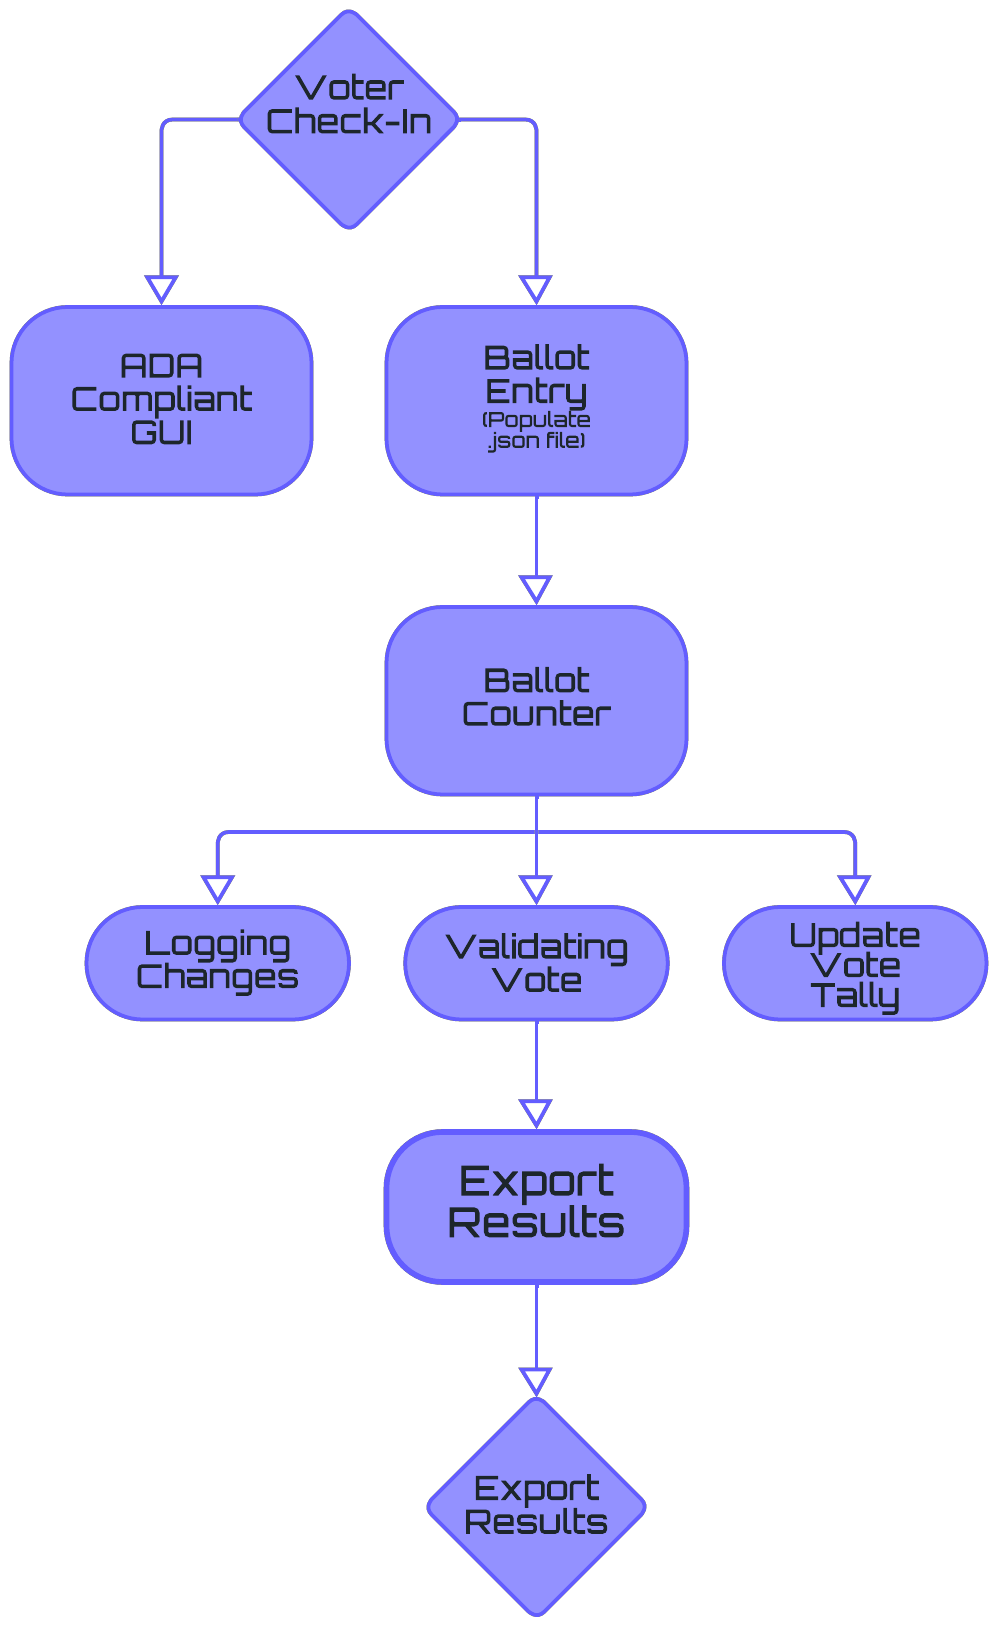
\includegraphics[width=0.5\textwidth]{docs/sad/figures/architecture.png}
\caption{System Architecture}
\label{fig:architecture}
\end{wrapfigure}

The Architecture Design Overview section meticulously maps out the journey within the New Mexico Voting Simulation system, from voter check-in to the final act of casting a vote, as systematically depicted in Figure \ref{fig:architecture}. The figure serves as a visual aid, outlining the flow and interplay between modules such as the ADA Compliant \gls{GUI}\footnote{\glsdesc{GUI}} and the Ballot Counter, illustrating a network of processes that are both interdependent and integral to the electoral system. This section aims to elucidate the logical sequence and purposeful design of each module, underpinning the system’s integrity and operational efficiency. \\ \\
Starting with the Voter Check-In module, we trace the voter’s path through the system, noting how each module is tailored to facilitate specific aspects of the voting process. The ADA Compliant GUI, for instance, is not just a point of interaction but a gateway through which voters’ preferences are securely logged and converted into structured \gls{json}\footnote{\glsdesc{json}} format, ready for subsequent stages of data handling. As highlighted in Figure \ref{fig:architecture}, the attention to detail in this workflow is critical, ensuring that voter data flows seamlessly and securely through the system, maintaining the integrity of each vote. \\ \\
Expanding upon the Overview, we will delve deeper into the subsequent sections, which discuss the Voter Interface and Flow, Data Management and Integrity, and System Output and Result Dissemination in comprehensive detail. Each section is dedicated to a specific aspect of the system's architecture, providing a granular look at the functionalities that ensure a transparent and accurate voting process, supported by the reliability of the system’s design.

\clearpage

\subsection{Voter Interface and Flow}
Analyzing the Voter Interface and Flow, we delve into the Voter Check-In and ADA \cite{adaVotingPolling} Compliant GUI's intricate design aspects, as depicted in Figure \ref{fig:architecture}. The GUI is engineered to provide an accessible and intuitive voting experience. In Figure \ref{fig:accessibility}, we see the Accessibility Selection Interface, which illustrates the thoughtful integration of options like larger text, high contrast modes, and text-to-speech capabilities. These features are not merely about compliance but are core to our design philosophy, ensuring that every voter can navigate the system with independence and ease. As voters interact with the system, their selections are methodically captured. This precise process, from \gls{authentication}\footnote{\glsdesc{authentication}} to the final vote confirmation, is central to the design, ensuring a seamless flow that is both intuitive and secure. The real-time capture of voter actions facilitates a smooth transition to subsequent stages in the voting process.

\begin{figure}[h]
  \centering
  \begin{minipage}[b]{0.4\textwidth}
    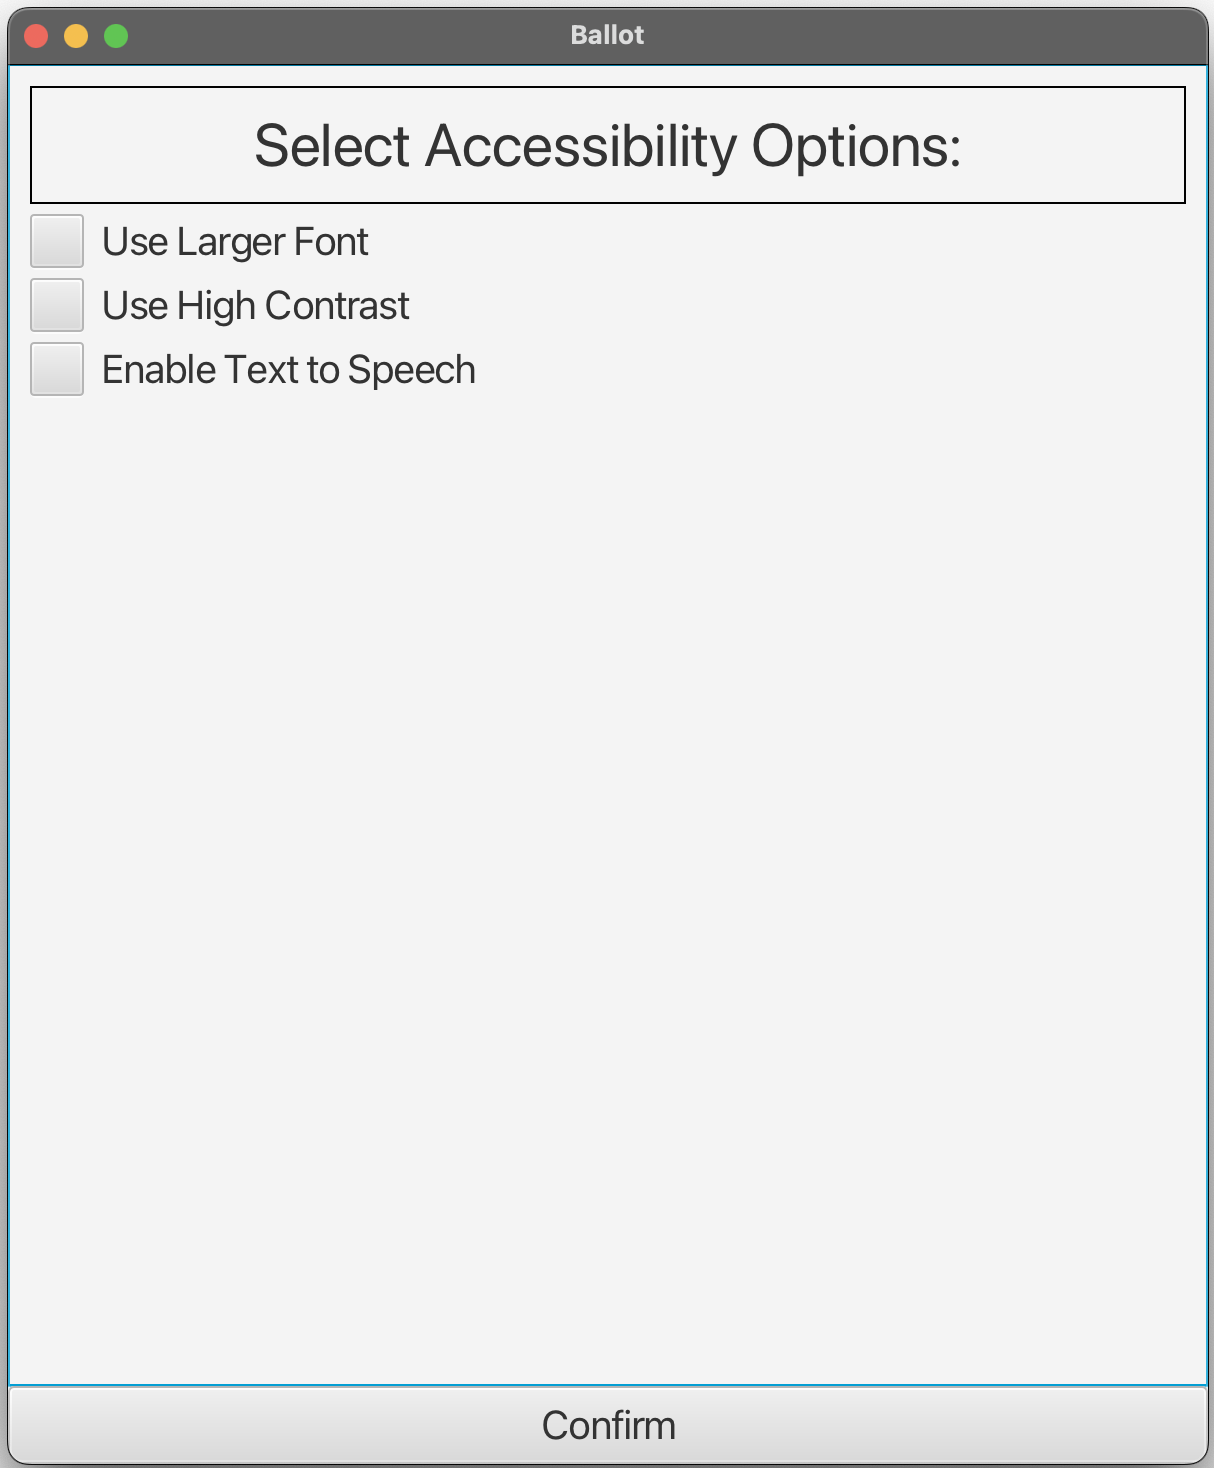
\includegraphics[width=\textwidth]{docs/sad/figures/accessibility.png}
    \caption{Accessibility Selection Interface}
    \label{fig:accessibility}
  \end{minipage}
  \hfill
  \begin{minipage}[b]{0.4\textwidth}
    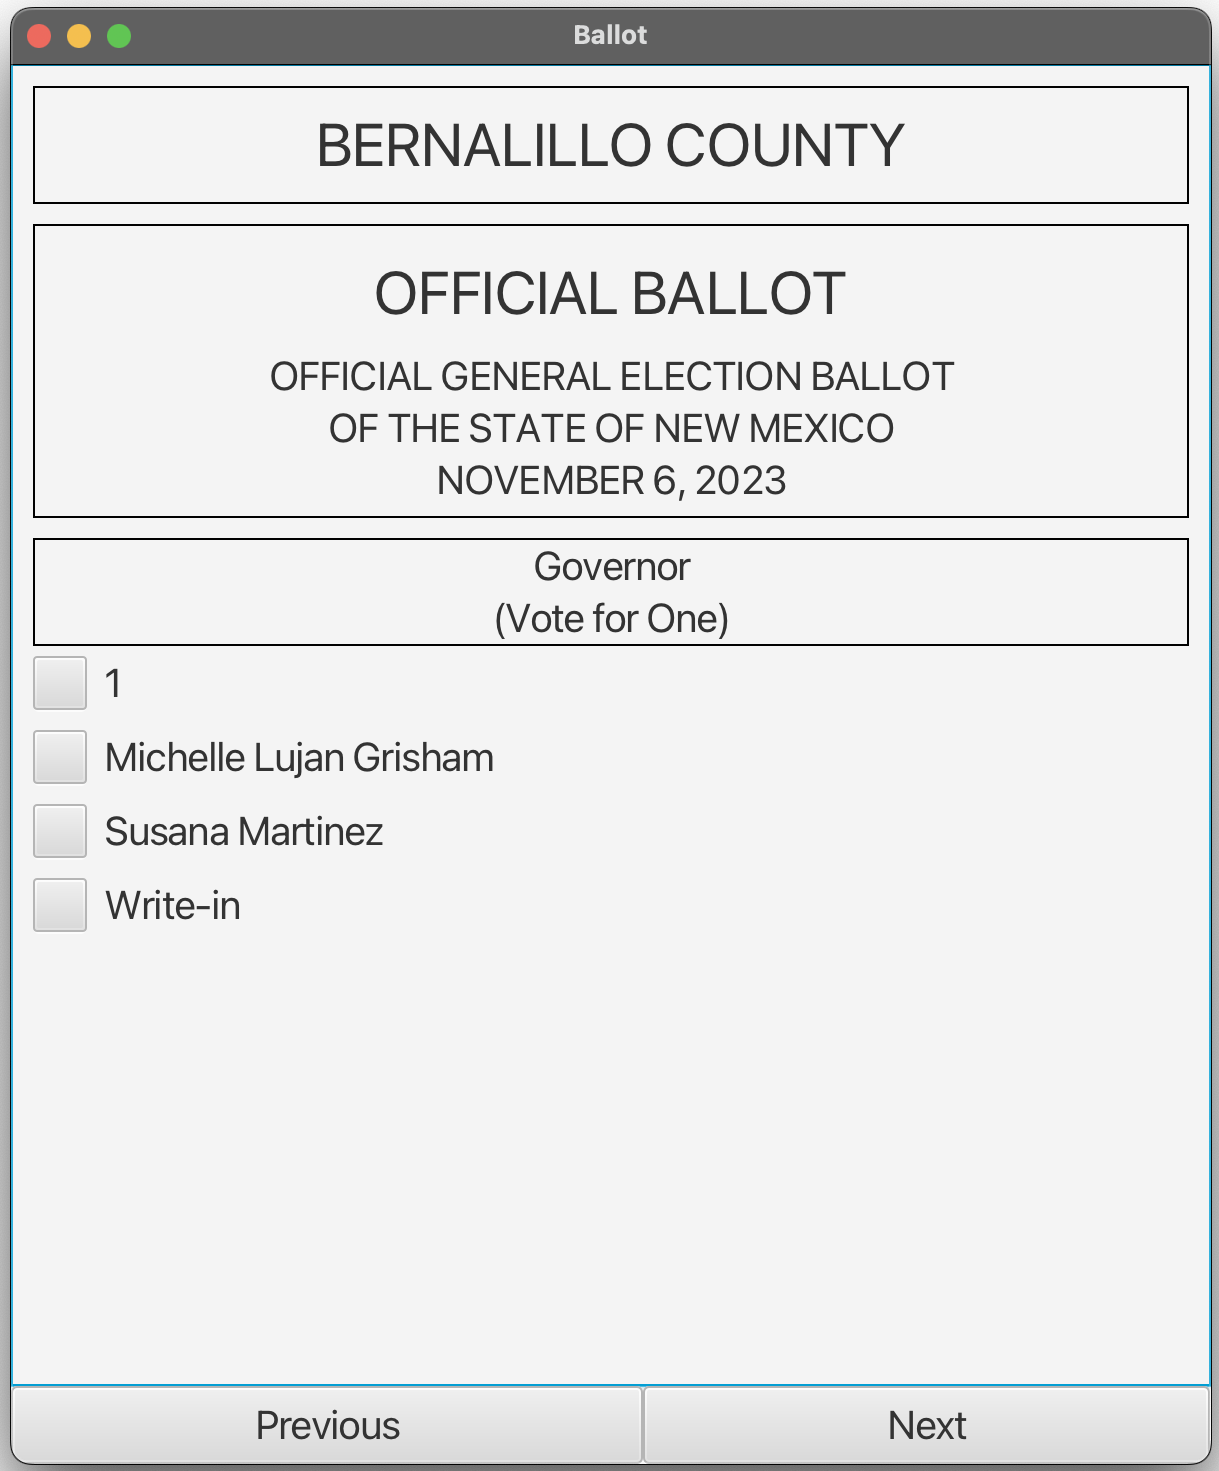
\includegraphics[width=\textwidth]{docs/sad/figures/ballot.png}
    \caption{Ballot Interface}
    \label{fig:ballot}
  \end{minipage}
\end{figure}

\subsection{Data Management and Integrity}
The strategic adoption of JSON files is discussed in this subsection, focusing on their role in enhancing data security and integrity within the Voting Simulation system. JSON files are chosen for their readability and ease of use, which are crucial for the \gls{audit}\footnote{\glsdesc{audit}} process and ensuring data integrity, as outlined in Figure \ref{fig:architecture}'s workflow. Each vote is \gls{encapsulate}\footnote{\glsdesc{encapsulate}} as a JSON object, creating a reliable and discrete record of the voter's intent. This approach not only secures data in transit but also fortifies storage, with JSON's structured nature allowing for automated validation processes that are essential for maintaining the voting system’s transparency. The integrity of these files is paramount, and their role in the system extends beyond mere storage—they are foundational to the Voting Simulation system's ability to provide a trustworthy framework for the entire electoral process.

\subsection{System Output and Result Dissemination}
The role of the BallotCounterGUI in the tabulation and dissemination of results is paramount, as it transforms the individual votes into an \gls{aggregate}\footnote{\glsdesc{aggregate}} format suitable for analysis and presentation. This GUI is a critical component of the system's architecture, ensuring that the vote counts are not only tallied but also visually represented in an easily interpretable format for stakeholders, as shown in Figure 
\ref{fig:counter}. The process of converting these votes into a comprehensible output is integral to the system's function, providing election officials and the public with clear, understandable results. The 
BallotCounterGUI interacts with the underlying JSON data to ensure accurate and real-time results are presented, highlighting the system’s capability in managing the \gls{end-to-end}\footnote{\glsdesc{end-to-end}} process from vote casting to result dissemination.

\begin{figure}[h]
    \centering
    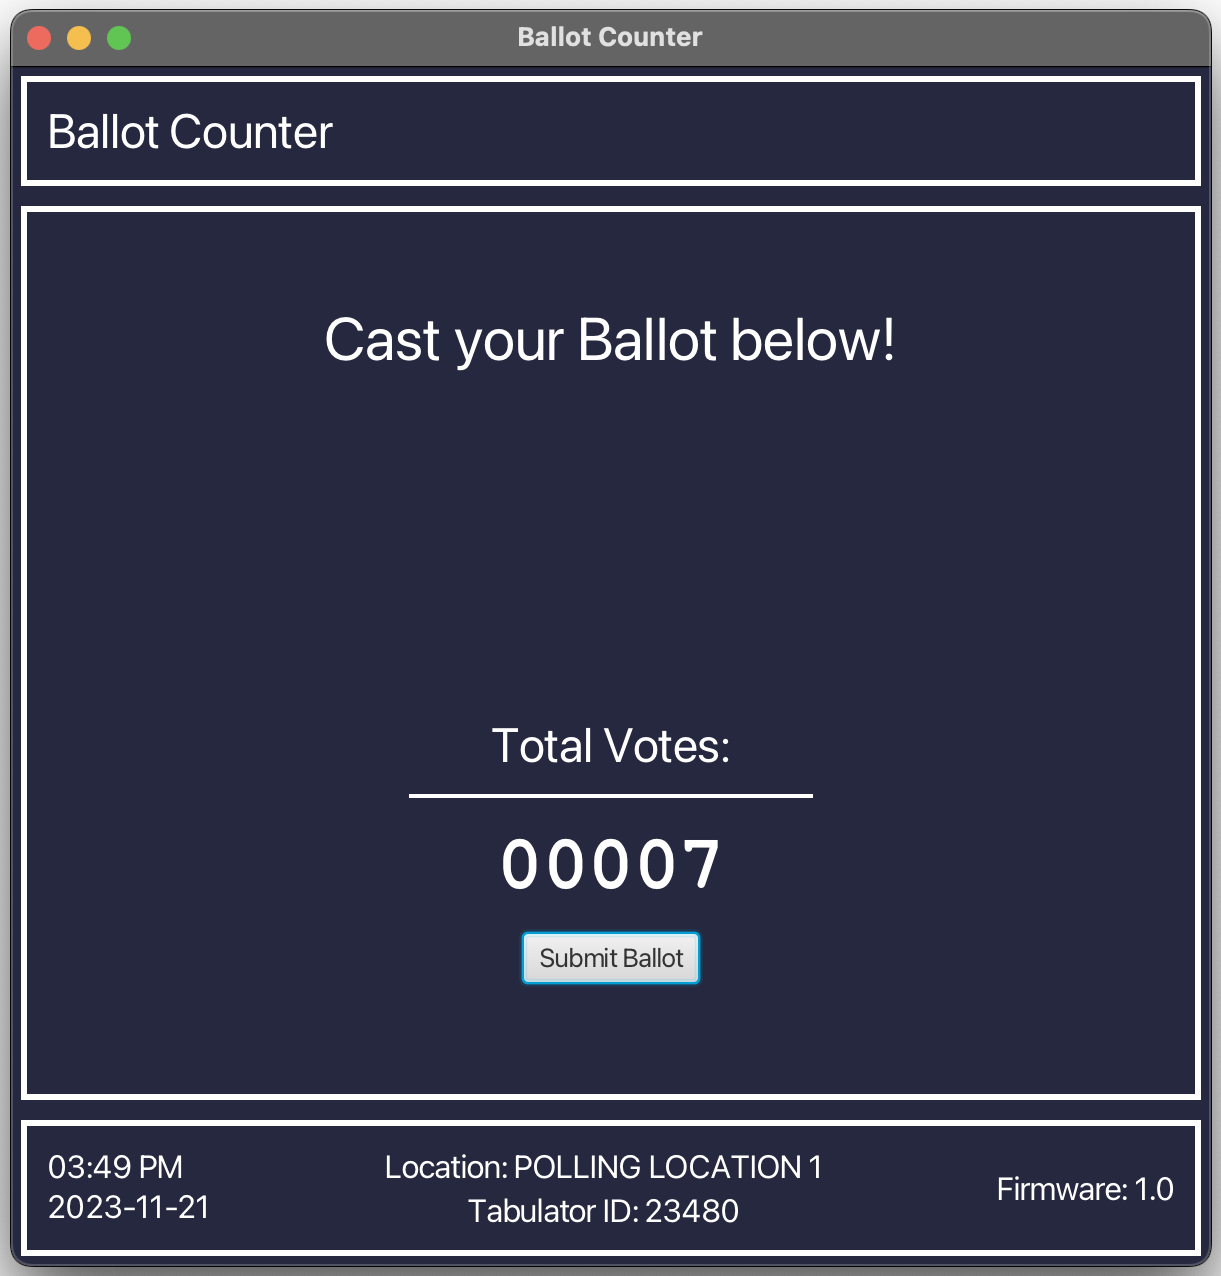
\includegraphics[scale=0.3]{docs/sad/figures/counter.png}
    \caption{Vote Counter}
    \label{fig:counter}
\end{figure}

\section{Component Specifications}
This section delves into the detailed architecture of the New Mexico Voting Simulation system, articulating the pivotal roles and interactivity of each component. It commences with an analysis of the Ballot component, which encompasses the \textit{BallotResult} class — a dynamic repository for individual voting outcomes, and the \textit{PositionResult} class, tasked with the precise recording of voters' selections. These classes are instrumental in maintaining the integrity of the voting process, providing the foundation for reliable vote tallying and the subsequent stages of result verification. \\ \\
Following this, the section examines the Regulation component, which includes the \textit{CheckInGUI} and \textit{Register} classes, fundamental to ensuring voter eligibility and the integrity of the electoral roll. The \textit{TestRegistration} class underscores the system's robust pre-election testing, ensuring functionality and accuracy before deployment. The final piece of the architectural puzzle is the Tabulation component, highlighted by the \textit{BallotCounterGUI}, which is depicted in Figure \ref{fig:counter}. This interface is crucial in translating individual ballots into aggregated election results, offering real-time updates and transparent reporting, thus reinforcing the system's dedication to delivering an election process that is both trustworthy and verifiable.

\subsection{Ballot}
Here, we aim to give a foundation to understanding how the system handles the core element of any election—the vote. It describes the \textit{BallotResult} class, which serves as a vessel for the election outcomes for different positions. It also outlines the dynamic addition of results as new positions are introduced throughout the election lifecycle. This class is crucial for accumulating and storing vote data, which is later utilized for result tabulation and verification. The \textit{PositionResult} class, intricately linked to \textit{BallotResult}, tracks the candidates and records voter choices, ensuring a direct and error-free translation of voter intent into the system.

\subsubsection{BallotResult}
The \textit{BallotResult} class is designed to encapsulate and manage the results of voting for different positions on a ballot. This class serves as a container for the results of individual voting positions. It allows the dynamic addition of results for new positions as the voting progresses. The \textit{BallotResult} class would be used in the context of accumulating the results after voters have cast their votes. Each \textit{PositionResult} associated with a specific ballot position (such as "President", "Senator", etc.) is stored with a corresponding position label. \\ \\
\textbf{Dependencies}

\begin{itemize}
    \item PositionResult: This class depends on the \textit{PositionResult} class, which should be defined to hold the result data for individual positions.
\end{itemize}

\subsubsection{PositionResult}
The \textit{PositionResult} class is responsible for tracking the candidates for a particular position on the ballot and recording the voter's choice. It allows for the addition and retrieval of candidates for a specific position. It also stores the chosen candidate from the list of candidates for an individual voter. The \textit{PositionResult} class is used whenever there is a need to manage candidates for a specific position and to store or update the voter's selection. For example, after a voter selects their candidate in the GUI, the \textit{PositionResult} would record this choice.

\begin{itemize}
    \item addCandidate(String candidate): Adds a candidate's name to the list of candidates for a voting position.
    \item getCandidates(): Retrieves the list of candidates.
    \item setCandidates(List$<$String$>$ candidates): Sets the list of candidates to a new list.
    \item getVoterChoice(): Gets the voter's selected candidate.
    \item setVoterChoice(String voterChoice): Records the voter's selected candidate.
\end{itemize}

\subsubsection{TextToSpeech}
The \textit{TextToSpeech} class provides an auditory representation of text, intended to assist visually impaired voters or to articulate text-based information within the voting system. It converts provided text into audible speech, allocates the necessary resources to enable speech synthesis and delivers the spoken output of the given text using the \textit{FreeTTS} library. The \textit{TextToSpeech} class is intended for use in situations where the voting system needs to provide audible feedback or instructions to the user, enhancing accessibility.\\ \\
\textbf{Dependencies}

\begin{itemize}
    \item FreeTTS: Depends on the \textit{FreeTTS} library and specifically requires the "Kevin" voice directory for its functionality.
\end{itemize}

\subsubsection{VoteFormGUI}
The \textit{VoteFormGUI} class is designed to provide the graphical user interface for voters to interact with when casting their votes. It renders the voting form on the screen, displaying options for various ballot positions and candidates, Captures user inputs as they select their choices on the voting form, and it ensures that the voter's selections comply with the rules of the voting system, such as preventing over-voting.

\begin{itemize}
    \item initializeComponents(): Sets up the GUI components like buttons, labels, and input fields.
    \item displayCandidates(List$<$String$>$ candidates): Shows the list of candidates to the voter.
    \item recordVote(String candidate): Records the voter's choice.
    \item confirmSelection(): Provides a confirmation dialog to the voter to verify their selection.
    \item showResults(Map$<$String, Integer$>$ results): Displays the voting results to the voter or election officials.
    \item printBallot(): Initiates the printing of the voter's ballot for verification purposes, if required by law.
    \item generateReport(): Generates an electronic data file of the voting session for record-keeping and auditing.
\end{itemize}
\textbf{Dependencies}

\begin{itemize}
    \item VotingController: Interacts with the \textit{VotingController} to process the votes and handle the logic.
    \item TextToSpeech: Could potentially use the \textit{TextToSpeech} class to assist voters with visual impairments.
\end{itemize}

\subsubsection{VotingController}
The \textit{VotingController} class serves as the central logic controller for the voting process, managing the selection of candidates for various offices, tabulating results, and persisting data. It initializes the list of offices and their corresponding candidates, manages a voting session, including voter selections for different positions, aggregates and tabulates the results of the voting session and converts the voting results into a JSON format and saves them to a .json file.

\begin{itemize}
    \item VotingController(): Constructor that initializes the \textit{ballotResult} object and sets up the offices and candidates.
    \item initializeOffices(): Populates the offices list with predefined offices and their candidates.
    \item getOffices(): Returns the list of offices and candidates.
    \item selectionContainsKey(String position): Checks if a selection has been made for a given position.
    \item getCandidatesForPosition(String position): Retrieves the candidates for a specific office based on the voter’s selection.
    \item handleSubmit(): Finalizes the voting process by tabulating results, printing them to the console, and saving to a .json file.
    \item saveSelection(String position, String s): Records a voter’s selection for a given position.
\end{itemize}
\textbf{Dependencies}

\begin{itemize}
    \item Gson: Requires the \textit{Gson} library for .json serialization.
    \item BallotResult: Depends on the \textit{BallotResult} class to hold and manage the overall voting results.
    \item PositionResult: Utilizes the \textit{PositionResult} class to manage individual voting results for each position.
\end{itemize}

\subsection{Regulation}
The Regulation subsection details the essential controls and checks that ensure the voting process adheres to legal and procedural standards. The \textit{CheckInGUI} class, which features prominently in this subsection, offers a detailed look at the check-in interface, where eligibility is confirmed, and voter details are meticulously verified. The Register class, pivotal to voter management, is explored for its role in voter registration and verification, acting as a gatekeeper to prevent unauthorized or duplicate voting. The \textit{TestRegistration} class demonstrates the system’s commitment to reliability, simulating the registration process to test and validate the system before live deployment.

\subsubsection{CheckInGUI}
The \textit{CheckInGUI} class provides a user interface for the check-in process of voters within the voting system. It is responsible for gathering voter information and validating their eligibility to vote.
It presents form fields for voter information entry, such as name, address, SSN, and date of birth, validates the input fields to ensure that all necessary information is filled in correctly, converts the date of birth input into a \textit{LocalDate} object using the specified format and  Handles the logic to check in a voter, including verifying registration and whether the voter has already voted.

\begin{itemize}
    \item start(Stage primaryStage): Initializes the GUI components and sets up the primary stage of the application.
    \item createGridPane(): Constructs the layout for the UI controls.
    \item addUIControls(GridPane grid): Adds labels, text fields, and buttons to the grid pane.
    \item createCheckInButton(): Creates a styled button for the check-in action.
    \item handleCheckInAction(): Invoked when the check-in button is clicked, processes the voter’s check-in.
    \item areFieldsValid(String...): Validates the input fields for completeness.
    \item parseDateOfBirth(String dobString): Attempts to parse the provided date of birth string into a LocalDate object.
    \item processCheckIn(String, String, String, String, LocalDate): Processes the voter check-in if all validations pass.
    \item createVoterID(String, String, String, LocalDate): Generates a voter ID based on the provided information.
\end{itemize}
\textbf{Dependencies}

\begin{itemize}
    \item Register: Interacts with the Register class to verify voter registration and check-in status.
\end{itemize}

\subsubsection{Register}
The \textit{Register} class manages the registration and verification of voters. It is responsible for maintaining a list of registered voters, checking in voters, and persisting voter information. It allows new voters to be registered and added to the system, searches for and retrieves voter information based on identifying details, marks a voter as having voted and prevents re-voting and saves and loads the registered voters' data from a file.

\begin{itemize}
    \item Register(): Constructor that loads the list of registered voters from a file upon instantiation.
    \item registerVoter(Voter newVoter): Registers a new voter if they are not already registered.
    \item findVoter(String firstName, String lastName, String ssnLast4, String address, LocalDate dob): Looks up a voter based on personal information.
    \item checkInVoter(String firstName, String lastName, String ssnLast4, String address, LocalDate dob): Checks in a voter on election day, ensuring they have not already voted.
    \item saveToFile(): Saves the current state of registered voters to a file.
    \item isRegistered(String voterID): Checks if a voter is already registered based on their voter ID.
    \item printVoters(): Prints the details of all registered voters to the console for verification.
\end{itemize}
\textbf{Dependencies}

\begin{itemize}
    \item Voter: Relies on the Voter class to represent individual voter data.
\end{itemize}

\subsubsection{TestRegistration}
The \textit{TestRegistration} class is designed to test the registration functionality of the voting system. It ensures that the \textit{Register} class can successfully add new voters to the system. This class instantiates Voter objects with test data, and uses the \textit{Register} class to add voters to the registry. Creates instances of \textit{Voter}, initializes the \textit{Register} class, and registers voters for testing purposes.
\textbf{Dependencies}
\begin{itemize}
    \item Register: Depends on the \textit{Register} class to perform the registration actions.
    \item Voter: Utilizes the \textit{Voter} class to create test voter instances.
\end{itemize}

\subsubsection{Voter}
The \textit{Voter} class represents an individual voter within the system, storing personal and voting-specific information. It holds information such as the voter's full name, address, date of birth, and last four digits of their SSN, keeps track of whether the voter has already voted, generates a unique voter ID based on the voter's personal information and it offers a method to check if a set of given details matches the voter's information. This class plays a critical role in ensuring the accuracy and integrity of the voter registration and verification process within the voting simulation system.

\begin{itemize}
    \item Voter(String fullName, String address, LocalDate dateOfBirth, String ssnLastFour): Constructor that initializes the voter's details and generates a unique ID.
    \item getVoterID(): Returns the voter's unique ID.
    \item getFullName(): Retrieves the voter's full name.
    \item getAddress(): Retrieves the voter's address.
    \item getDateOfBirth(): Retrieves the voter's date of birth.
    \item getSsnLastFour(): Retrieves the last four digits of the voter's SSN.
    \item hasVoted(): Checks if the voter has already voted.
    \item markAsVoted(): Marks the voter as having voted.
    \item matches(String fullName, String address, LocalDate dob, String ssnLastFour): Checks if provided details match the voter's information.
\end{itemize}

\subsection{Tabulation}
In the Tabulation subsection, the spotlight is on the \textit{BallotCounterGUI}, which is depicted in Figure \ref{fig:counter}. This class represents the public face of the election results, converting individual votes into aggregate totals that are both accessible and comprehensible. Here, the focus is on the presentation of real-time voting data, reflecting the system's ability to not just collect but also dynamically display the ongoing results. The process described ensures transparency and timeliness in relaying the election progress to observers and participants alike.

\subsubsection{BallotCounterGUI}
The \textit{BallotCounterGUI} class provides a GUI for displaying and interacting with the ballot counting process. It is designed to present real-time voting data and system status information. It displays the current time and date, shows the total number of votes counted, provides a button for submitting ballots and also shows details like polling location, tabulator ID, and firmware version.

\begin{itemize}
    \item start(Stage primaryStage): Initializes the main window and sets up the layout and components of the GUI.
    \item createHeader(): Constructs the header section of the GUI.
    \item createVoteCounter(): Builds the central vote counter section.
    \item createFooter(): Creates the footer section with system information and real-time clock.
    \item startClock(): Initiates the real-time clock display.
    \item updateTime(): Updates the time and date display at regular intervals.
\end{itemize}

\section{Sample Use Cases}
Add overview of use cases here...

\subsection{Use Case 1}
Overview of Use Case 1 here...

\begin{itemize}
    \item \textbf{Actor}: User
    \item \textbf{Goal}: Stuff and things...
    \item \textbf{Preconditions}: Stuff and things...
    \item \textbf{Trigger}: Stuff and things...
    \item \textbf{Scenario}: Stuff and things...
    \begin{enumerate}
    \item \textbf{First Step}: Stuff and things...
    \item \textbf{Second Step}: Stuff and things...
    \item \textbf{Third Step}: Stuff and things...
    \item \textbf{Fourth Step}: Stuff and things...
    \end{enumerate}
\end{itemize}

\subsection{Use Case 2}
Overview of Use Case 2 here...

\begin{itemize}
    \item \textbf{Actor}: User
    \item \textbf{Goal}: Stuff and things...
    \item \textbf{Preconditions}: Stuff and things...
    \item \textbf{Trigger}: Stuff and things...
    \item \textbf{Scenario}: Stuff and things...
    \begin{enumerate}
    \item \textbf{First Step}: Stuff and things...
    \item \textbf{Second Step}: Stuff and things...
    \item \textbf{Third Step}: Stuff and things...
    \item \textbf{Fourth Step}: Stuff and things...
    \end{enumerate}
\end{itemize}

\subsection{Use Case 3}
Overview of Use Case 3 here...

\begin{itemize}
    \item \textbf{Actor}: User
    \item \textbf{Goal}: Stuff and things...
    \item \textbf{Preconditions}: Stuff and things...
    \item \textbf{Trigger}: Stuff and things...
    \item \textbf{Scenario}: Stuff and things...
    \begin{enumerate}
    \item \textbf{First Step}: Stuff and things...
    \item \textbf{Second Step}: Stuff and things...
    \item \textbf{Third Step}: Stuff and things...
    \item \textbf{Fourth Step}: Stuff and things...
    \end{enumerate}
\end{itemize}

\newpage

\printbibliography

{\parindent0pt}

\end{document}
